% ============================================================
%  يُترجَم بـ XeLaTeX  (في Overleaf: Menu → Compiler → XeLaTeX)
%  الخط: Amiri (متوفر في Overleaf، أو حمّله من github.com/aliftype/amiri)
% ============================================================
\documentclass[12pt,a4paper]{article}
\usepackage[a4paper,margin=1.7cm,top=2.3cm,bottom=2.9cm,headheight=15pt,footskip=1.5cm]{geometry}
\usepackage{amsmath,amssymb}
\usepackage{icomma}
\usepackage[english,bidi=default,layout=lists]{babel}
\babelprovide[import,main]{arabic}
\babelfont{rm}[Scale=1.08]{Amiri}
\babelfont{sf}[Scale=1.08]{Amiri}
\usepackage[most]{tcolorbox}
\usepackage{tikz}
\usetikzlibrary{arrows.meta,calc,shadings,shapes.misc}
\usepackage{array}
\usepackage{colortbl}
\usepackage{fancyhdr}
\usepackage{titlesec}
\usepackage{enumitem}
\usepackage{collcell}
\usepackage{needspace}
\usepackage{etoolbox}
\newcolumntype{C}{>{\collectcell\ar}c<{\endcollectcell}}
\pretocmd{\section}{\Needspace{15\baselineskip}}{}{}
\pretocmd{\subsection}{\Needspace{11\baselineskip}}{}{}

\definecolor{cDef}{HTML}{1F4E9C}
\definecolor{cThm}{HTML}{B3261E}
\definecolor{cRem}{HTML}{2E7D32}
\definecolor{cEx}{HTML}{C76B00}
\definecolor{cMeth}{HTML}{6A1B9A}
\definecolor{cSol}{HTML}{00695C}
\definecolor{cSec}{HTML}{1F3A68}

\titleformat{\section}{\Large\bfseries\color{cSec}}{\thesection.}{0.6em}{}[{\color{cSec!60}\titlerule[1pt]}]
\titleformat{\subsection}{\large\bfseries\color{cThm!85!black}}{\thesubsection.}{0.5em}{}
\titlespacing*{\section}{0pt}{14pt}{8pt}
\titlespacing*{\subsection}{0pt}{10pt}{5pt}
\setlength{\parindent}{0pt}
\setlength{\parskip}{4pt}
\setlist{itemsep=2pt,topsep=3pt}

\newtcolorbox{arbox}[3][]{enhanced,
  colback=#2!5,colframe=#2!80!black,arc=2mm,boxrule=0.8pt,
  left=6pt,right=6pt,top=8pt,bottom=5pt,
  fonttitle=\bfseries,coltitle=white,
  title={\foreignlanguage{arabic}{#3}},
  attach boxed title to top right={xshift=-5mm,yshift=-3mm},
  boxed title style={colback=#2!80!black,arc=1.5mm,boxrule=0pt},
  before upper={\selectlanguage{arabic}},
  before skip=8pt,after skip=8pt,breakable,#1}
\newenvironment{BOX}[2]{\begin{otherlanguage}{english}\begin{arbox}{#1}{#2}}{\end{arbox}\end{otherlanguage}}
\newenvironment{tarif}[1][تعريف]{\begin{BOX}{cDef}{#1}}{\end{BOX}}
\newenvironment{khassia}[1][خاصية]{\begin{BOX}{cThm}{#1}}{\end{BOX}}
\newenvironment{molahada}[1][ملاحظة]{\begin{BOX}{cRem}{#1}}{\end{BOX}}
\newenvironment{mithal}[1][مثال]{\begin{BOX}{cEx}{#1}}{\end{BOX}}
\newenvironment{tariqa}[1][طريقة]{\begin{BOX}{cMeth}{#1}}{\end{BOX}}

\newcounter{exo}
\newenvironment{tamrin}[1]{\stepcounter{exo}\begin{BOX}{cSec}{التمرين \theexo: #1}}{\end{BOX}}
\newenvironment{hal}{\Needspace{12\baselineskip}\begin{otherlanguage}{english}\begin{arbox}[breakable]{cSol}{حل التمرين \theexo}}{\end{arbox}\end{otherlanguage}}

\newenvironment{LTR}{\begin{otherlanguage}{english}}{\end{otherlanguage}}
\newcommand{\ar}[1]{\foreignlanguage{arabic}{#1}}

\renewcommand{\dots}{\mathinner{\ldotp\ldotp\ldotp}}
\renewcommand{\ldots}{\mathinner{\ldotp\ldotp\ldotp}}
\renewcommand{\cdots}{\mathinner{\cdotp\cdotp\cdotp}}
\newcommand{\N}{\mathbb{N}}
\newcommand{\Z}{\mathbb{Z}}
\newcommand{\D}{\mathbb{D}}
\newcommand{\Q}{\mathbb{Q}}
\newcommand{\R}{\mathbb{R}}
\newcommand{\pgcd}{\operatorname{PGCD}}
\newcommand{\ppcm}{\operatorname{PPCM}}

% \NLseg{a}{b}{[}{]} ; \NLright{a}{[} ; \NLleft{b}{]}  (interval on a number line)
\newcommand{\NLseg}[4]{\begin{LTR}\begin{tikzpicture}[baseline=-0.6ex]
 \draw[-{Stealth[length=2mm]},gray!70](0,0)--(3.4,0);
 \draw[line width=2pt,cThm!80!black](0.7,0)--(2.7,0);
 \node[cThm!80!black,font=\LARGE] at (0.7,0){$#3$};
 \node[cThm!80!black,font=\LARGE] at (2.7,0){$#4$};
 \node[below=3pt,font=\footnotesize] at (0.7,0){$#1$};
 \node[below=3pt,font=\footnotesize] at (2.7,0){$#2$};
\end{tikzpicture}\end{LTR}}
\newcommand{\NLright}[2]{\begin{LTR}\begin{tikzpicture}[baseline=-0.6ex]
 \draw[-{Stealth[length=2mm]},gray!70](0,0)--(3.4,0);
 \draw[line width=2pt,cThm!80!black](1.3,0)--(3.3,0);
 \node[cThm!80!black,font=\LARGE] at (1.3,0){$#2$};
 \node[below=3pt,font=\footnotesize] at (1.3,0){$#1$};
\end{tikzpicture}\end{LTR}}
\newcommand{\NLleft}[2]{\begin{LTR}\begin{tikzpicture}[baseline=-0.6ex]
 \draw[-{Stealth[length=2mm]},gray!70](0,0)--(3.4,0);
 \draw[line width=2pt,cThm!80!black](0.05,0)--(2.1,0);
 \node[cThm!80!black,font=\LARGE] at (2.1,0){$#2$};
 \node[below=3pt,font=\footnotesize] at (2.1,0){$#1$};
\end{tikzpicture}\end{LTR}}

% ---------- social-media icons (pure TikZ) ----------
\definecolor{cFB}{HTML}{1877F2}
\definecolor{cTG}{HTML}{229ED9}
\definecolor{cIG1}{HTML}{FEDA75}
\definecolor{cIG2}{HTML}{D62976}
\definecolor{cIG3}{HTML}{4F5BD5}
\newcommand{\fbicon}{\begin{LTR}\begin{tikzpicture}[baseline=-0.75ex,x=1em,y=1em]
 \fill[cFB] (0,0) circle (0.55);
 \node[white,inner sep=0,font=\usefont{TU}{lmss}{bx}{n}\small] at (0.04,-0.02) {f};
\end{tikzpicture}\end{LTR}}
\newcommand{\igicon}{\begin{LTR}
\begin{tikzpicture}[baseline=-0.75ex,x=1em,y=1em]
 \shade[lower left=cIG1,lower right=cIG2,upper left=cIG2,upper right=cIG3,rounded corners=0.28em] (-0.55,-0.55) rectangle (0.55,0.55);
 \draw[white,line width=0.09em,rounded corners=0.18em] (-0.36,-0.36) rectangle (0.36,0.36);
 \draw[white,line width=0.09em] (0,0) circle (0.17);
 \fill[white] (0.22,0.22) circle (0.05);
\end{tikzpicture}\end{LTR}}
\newcommand{\tgicon}{\begin{LTR}
\begin{tikzpicture}[baseline=-0.75ex,x=1em,y=1em]
 \fill[cTG] (0,0) circle (0.55);
 \fill[white] (-0.33,0.0) -- (0.32,0.27) -- (0.2,-0.3) -- (0.0,-0.15) -- (-0.08,-0.28) -- (-0.08,-0.08) -- cycle;
 \fill[cTG!70!black] (-0.08,-0.08) -- (0.25,0.2) -- (0.0,-0.15) -- (-0.08,-0.28) -- cycle;
\end{tikzpicture}\end{LTR}}
% page number: black box, white two-digit number, at the right of the social row
\newcommand{\PageBox}{\begin{LTR}\tikz[baseline=(p.base)]\node[fill=black,text=white,inner sep=2.5pt,minimum width=1.6em,minimum height=1.3em,font=\usefont{TU}{lmss}{bx}{n}\small](p){\ifnum\value{page}<10 0\fi\arabic{page}};\end{LTR}}
% visual left-to-right order: Telegram | Instagram | Facebook | page box
\newcommand{\SocialRow}{\begin{otherlanguage}{english}%
 \ar{\textbf{الأستاذ سوايسية هشام للرياضيات}}\ \tgicon\hfill
 \textbf{prof\_hicham\_math}\ \igicon\hfill
 \ar{\textbf{الأستاذ سوايسية هشام للرياضيات}}\ \fbicon\hspace{2.2em}\PageBox\end{otherlanguage}}

\pagestyle{fancy}
\fancyhf{}
\renewcommand{\headrulewidth}{0.6pt}
\renewcommand{\footrulewidth}{0.4pt}
% \SetHeader{right head: document title}{left head: level -- stream}
\newcommand{\SetHeader}[2]{%
 \fancyhead[C]{\parbox{\textwidth}{\ar{#1\hfill #2}}}%
 \fancyfoot[C]{\parbox{\textwidth}{\small\SocialRow}}}
\usepackage{tkz-tab}
\usepackage{multicol}
% variation / sign table (LTR)
\newenvironment{TAB}{\par\begin{center}\begin{LTR}\begin{tikzpicture}[scale=0.95,every node/.style={font=\small}]}{\end{tikzpicture}\end{LTR}\end{center}}
% grid + axes, clipped: \begin{GR}{xmin}{xmax}{ymin}{ymax}{unit cm}
\newenvironment{GR}[5]{\par\begin{center}\begin{LTR}\begin{tikzpicture}[x=#5cm,y=#5cm,font=\footnotesize]
 \draw[gray!25,very thin] (#1,#3) grid (#2,#4);
 \draw[-{Stealth[length=2mm]}] (#1,0)--(#2+0.3,0) node[below left]{$x$};
 \draw[-{Stealth[length=2mm]}] (0,#3)--(0,#4+0.3) node[below left]{$y$};
 \node[below left] at (0,0){$O$};
 \begin{scope}\clip (#1,#3) rectangle (#2,#4);}
{\end{scope}\end{tikzpicture}\end{LTR}\end{center}}
\newcommand{\Ticks}[2]{\foreach \t in {#1} \node[below,font=\scriptsize] at (\t,0){$\t$}; \foreach \t in {#2} \node[left,font=\scriptsize] at (0,\t){$\t$};}
\newcommand{\bx}[1]{\ensuremath{\colorbox{cDef!12}{$\displaystyle #1$}}}
\newcommand{\TwoCol}[4]{\par\begin{LTR}\noindent\begin{minipage}[t]{#1\textwidth}\selectlanguage{arabic}#2\end{minipage}\hfill\begin{minipage}[t]{#3\textwidth}\selectlanguage{arabic}#4\end{minipage}\end{LTR}\par}
\newcommand{\RL}[4]{\TwoCol{#3}{#4}{#1}{#2}}  % \RL{w1}{right content}{w2}{left content}
\newcommand{\ok}{$\textcolor{cRem}{\checkmark}$}
\newcommand{\limn}{\displaystyle\lim_{n\to+\infty}}
% sub-questions, each on its own line
\newenvironment{sq}{\begin{itemize}[leftmargin=2.4em,itemsep=3pt]}{\end{itemize}}
\newcommand{\qa}{\item[(أ)]}\newcommand{\qb}{\item[(ب)]}\newcommand{\qc}{\item[(جـ)]}\newcommand{\qd}{\item[(د)]}\newcommand{\qe}{\item[(هـ)]}
\newcommand{\pa}{\par\smallskip\textbf{(أ)} }\newcommand{\pb}{\par\smallskip\textbf{(ب)} }\newcommand{\pc}{\par\smallskip\textbf{(جـ)} }\newcommand{\pd}{\par\smallskip\textbf{(د)} }\newcommand{\pe}{\par\smallskip\textbf{(هـ)} }
\newcommand{\QQ}[1]{\par\smallskip\textbf{#1.} }
\newenvironment{tmr}{\stepcounter{exo}\begin{BOX}{cSec}{تمرين محلول \theexo}}{\end{BOX}}
\newcommand{\ABC}[3]{\\[2pt]\begin{tabular}{p{0.28\textwidth}p{0.28\textwidth}p{0.28\textwidth}}(جـ) \ #3 & (ب) \ #2 & (أ) \ #1\end{tabular}}
\pretocmd{\section}{\Needspace{24\baselineskip}}{}{}
\newtcbox{\bxtbox}{on line,colback=cDef!12,colframe=cDef!12,boxrule=0pt,arc=1pt,boxsep=0pt,left=2pt,right=2pt,top=1pt,bottom=1pt}
\newcommand{\bxt}[1]{\foreignlanguage{english}{\bxtbox{\ar{#1}}}}
\renewcommand{\bx}[1]{\ensuremath{\colorbox{cDef!12}{$\displaystyle\color{cThm}#1$}}}
\renewcommand{\bxt}[1]{\foreignlanguage{english}{\bxtbox{\ar{\color{cThm}#1}}}}
\newcommand{\LW}[1]{{\color{cDef}#1}}
\newcommand{\ck}{\ensuremath{{\color{cRem}\checkmark}}}
\newcommand{\Venn}[2]{\begin{tikzpicture}[scale=0.8]
 \draw[thick,rounded corners] (-2.4,-1.5) rectangle (2.4,1.5); \node at (-2.1,1.2){$\Omega$};
 \begin{scope}#1\end{scope}
 \draw[thick,cDef] (-0.55,0) circle (1); \draw[thick,cThm] (0.55,0) circle (1);
 \node[cDef] at (-1.2,0.95){$A$}; \node[cThm] at (1.2,0.95){$B$};
 \node[below,font=\small] at (0,-1.5){#2};
\end{tikzpicture}}
\SetHeader{\small\bfseries\color{cSec}ملخص: الاحتمالات}{\small\color{cSec}السنة الثالثة ثانوي -- تسيير واقتصاد}
\begin{document}
\begin{LTR}
\begin{tcolorbox}[enhanced,colback=cSec!10,colframe=cSec!40,arc=3mm,halign=center,boxrule=0.6pt,top=12pt,bottom=12pt,before upper={\selectlanguage{arabic}}]
{\color{cSec}\fontsize{28}{34}\selectfont\bfseries الاحتمالات}\\[8pt]
{\color{cSec!80!black}\large ملخص شامل مع أمثلة وأشكال وتمارين محلولة خطوة بخطوة}\\[5pt]
{\color{cSec!80!black}\large السنة الثالثة ثانوي -- شعبة تسيير واقتصاد}
\end{tcolorbox}
\end{LTR}

\begin{BOX}{cSec}{محتوى الملخص (حسب البرنامج والتوزيع السنوي: المحور 7 ، الأسابيع 23--26)}
\begin{multicols}{2}
\begin{enumerate}[label=\textbf{\arabic*.}]
\item تذكير: التجربة العشوائية والحوادث.
\item قانون احتمال على مجموعة منتهية.
\item المتغير العشوائي: قانونه ، أمله ، تباينه ، انحرافه المعياري.
\item الاحتمال الشرطي.
\item الشجرة المتوازنة وبناؤها.
\item دستور الاحتمالات الكلية.
\item استقلال حادثتين.
\item تمارين محلولة.
\item خلاصة الطرائق.
\end{enumerate}
\end{multicols}
\end{BOX}

%================================================================
\section{تذكير: التجربة العشوائية والحوادث}
\begin{tarif}
\begin{itemize}
\item \textbf{التجربة العشوائية:} تجربة نعرف كل نتائجها الممكنة ولا يمكن توقع النتيجة قبل إجرائها (رمي زهرة نرد ، سحب كرية من كيس ، اختيار شخص من مجموعة).
\item \textbf{مجموعة الإمكانيات} $\Omega$: مجموعة كل النتائج الممكنة ، ونرمز لعدد عناصرها بـ $\text{card}\,\Omega$.
\item \textbf{الحادثة:} كل جزء $A$ من $\Omega$. \ الحادثة \textbf{البسيطة} تحوي نتيجة واحدة ، و $\Omega$ \textbf{الحادثة الأكيدة} ، و $\varnothing$ \textbf{الحادثة المستحيلة}.
\end{itemize}
\end{tarif}
\begin{khassia}[العمليات على الحوادث]
\begin{itemize}
\item $A\cap B$ («$A$ و $B$»): تتحقق إذا تحققت $A$ و $B$ معًا.
\item $A\cup B$ («$A$ أو $B$»): تتحقق إذا تحققت إحداهما على الأقل.
\item $\overline A$ (الحادثة العكسية لـ $A$): تتحقق إذا لم تتحقق $A$.
\item $A$ و $B$ \textbf{غير متلائمتين} (متنافيتين) إذا كان $A\cap B=\varnothing$.
\end{itemize}
\begin{center}\begin{LTR}
\Venn{\clip (0.55,0) circle (1); \fill[cEx!35] (-0.55,0) circle (1);}{$A\cap B$}\quad
\Venn{\fill[cEx!35] (-0.55,0) circle (1); \fill[cEx!35] (0.55,0) circle (1);}{$A\cup B$}\quad
\Venn{\fill[cEx!35] (-2.4,-1.5) rectangle (2.4,1.5); \fill[white] (-0.55,0) circle (1);}{$\overline A$}
\end{LTR}\end{center}
\end{khassia}
\begin{mithal}
نرمي زهرة نرد مرقمة من $1$ إلى $6$: \ $\Omega=\{1;2;3;4;5;6\}$. نعتبر $A$: «الرقم زوجي» $=\{2;4;6\}$ و $B$: «الرقم أصغر من $3$» $=\{1;2\}$:
\[A\cap B=\{2\}\qquad;\qquad A\cup B=\{1;2;4;6\}\qquad;\qquad\overline A=\{1;3;5\}\]
\end{mithal}

%================================================================
\section{قانون احتمال على مجموعة منتهية}
\begin{tarif}
$\Omega=\{e_1;e_2;\ldots;e_n\}$ مجموعة إمكانيات تجربة عشوائية. نعرّف \textbf{قانون احتمال} على $\Omega$ بإرفاق كل نتيجة $e_i$ بعدد $p_i$ حيث:
\[\bx{0\leqslant p_i\leqslant1}\qquad;\qquad\bx{p_1+p_2+\cdots+p_n=1}\]
احتمال حادثة $A$ هو مجموع احتمالات النتائج التي تكوّنها ، ونرمز له بـ $P(A)$.
\end{tarif}
\begin{khassia}[خواص]
\[\LW{P(\varnothing)=0}\qquad\LW{P(\Omega)=1}\qquad\LW{0\leqslant P(A)\leqslant1}\qquad\LW{P\big(\overline A\big)=1-P(A)}\]
\[\LW{P(A\cup B)=P(A)+P(B)-P(A\cap B)}\]
وإذا كانت $A$ و $B$ غير متلائمتين: $\LW{P(A\cup B)=P(A)+P(B)}$.
\end{khassia}
\begin{khassia}[تساوي الاحتمال]
إذا كانت كل النتائج لها نفس الاحتمال (زهرة نرد غير مزيفة ، سحب عشوائي ، كريات متماثلة ، $\ldots$) فإن:
\[\bx{P(A)=\frac{\text{card}\,A}{\text{card}\,\Omega}}\]
أي: عدد الحالات الملائمة على عدد الحالات الممكنة.
\end{khassia}
\begin{mithal}[زهرة نرد مزيفة]
زهرة نرد مزيفة بحيث احتمال ظهور الوجه $k$ يتناسب مع $k$: $p_k=ak$.
\par $a+2a+3a+4a+5a+6a=1$ ، أي $21a=1$ ، ومنه \bx{a=\frac1{21}}.
\begin{center}\begin{LTR}\renewcommand{\arraystretch}{1.6}
\begin{tabular}{|C|c|c|c|c|c|c|c|}\hline
\rowcolor{cSec!12}الوجه $k$ & $1$ & $2$ & $3$ & $4$ & $5$ & $6$ & \ar{المجموع}\\\hline
$p_k$ & $\frac1{21}$ & $\frac2{21}$ & $\frac3{21}$ & $\frac4{21}$ & $\frac5{21}$ & $\frac6{21}$ & $1$\\\hline
\end{tabular}\end{LTR}\end{center}
احتمال ظهور رقم زوجي: $P=\dfrac{2+4+6}{21}=\dfrac{12}{21}=\bx{\frac47}$ \ ، واحتمال ظهور رقم فردي: $1-\dfrac47=\bx{\frac37}$.
\end{mithal}
\begin{mithal}[تجربة بمرحلتين: جدول ذو مدخلين]
نرمي قطعة نقدية متوازنة مرتين. نلخص النتائج في جدول ($F$: وجه ، $P$: ظهر):
\begin{center}\begin{LTR}\renewcommand{\arraystretch}{1.4}
\begin{tabular}{|c|c|c|}\hline
\rowcolor{cSec!12}\ar{الأولى}$\backslash$\ar{الثانية} & $F$ & $P$\\\hline
\cellcolor{cSec!12}$F$ & \cellcolor{cEx!25}$FF$ & $FP$\\\hline
\cellcolor{cSec!12}$P$ & $PF$ & $PP$\\\hline
\end{tabular}\end{LTR}\end{center}
$\text{card}\,\Omega=4$ ، واحتمال الحصول على وجهين: $\bx{\frac14}$ ، واحتمال الحصول على وجه واحد على الأقل: $1-P(PP)=\bx{\frac34}$.
\end{mithal}

%================================================================
\section{المتغير العشوائي}
\begin{tarif}
\textbf{المتغير العشوائي} $X$ هو دالة ترفق بكل نتيجة من $\Omega$ عددًا حقيقيًا (ربحًا ، خسارة ، عددًا ، $\ldots$).
\par \textbf{قانون احتمال} $X$: نعيّن القيم الممكنة $x_1$ ، $x_2$ ، $\ldots$ ، $x_n$ ، ثم الاحتمالات $p_i=P(X=x_i)$ في جدول ، و $p_1+p_2+\cdots+p_n=1$.
\end{tarif}
\begin{khassia}[الأمل الرياضياتي ، التباين ، الانحراف المعياري]
\[\bx{E(X)=x_1p_1+x_2p_2+\cdots+x_np_n}\]
\[\bx{V(X)=x_1^2p_1+x_2^2p_2+\cdots+x_n^2p_n-\big(E(X)\big)^2}\qquad\qquad\bx{\sigma(X)=\sqrt{V(X)}}\]
\textbf{تفسير} $E(X)$: متوسط القيم التي يأخذها $X$ إذا كررنا التجربة عددًا كبيرًا من المرات. في لعبة ربح: $E(X)>0$ اللعبة في صالح اللاعب ، $E(X)<0$ في غير صالحه ، $E(X)=0$ \textbf{لعبة عادلة}.
\end{khassia}
\begin{mithal}[لعبة يانصيب]
في كيس $10$ تذاكر: تذكرة واحدة تربح $20$ دينارًا ، و $3$ تذاكر تربح كل منها $5$ دنانير ، والباقي لا تربح شيئًا. ثمن المشاركة $4$ دنانير ، ونسحب تذكرة واحدة. $X$ الربح الصافي للاعب.
\par القيم: $20-4=16$ ، $5-4=1$ ، $0-4=-4$:
\begin{center}\begin{LTR}\renewcommand{\arraystretch}{1.5}
\begin{tabular}{|c|c|c|c|C|}\hline
\rowcolor{cSec!12}$x_i$ & $-4$ & $1$ & $16$ & المجموع\\\hline
$P(X=x_i)$ & $0{,}6$ & $0{,}3$ & $0{,}1$ & $1$\\\hline
\end{tabular}\end{LTR}\end{center}
\[E(X)=-4\times0{,}6+1\times0{,}3+16\times0{,}1=-2{,}4+0{,}3+1{,}6=\bx{-0{,}5}\]
$E(X)<0$: \bxt{اللعبة في غير صالح اللاعب} (يخسر في المتوسط $0{,}5$ دينار في كل مشاركة).
\[V(X)=16\times0{,}6+1\times0{,}3+256\times0{,}1-(-0{,}5)^2=35{,}5-0{,}25=\bx{35{,}25}\]
\[\sigma(X)=\sqrt{35{,}25}\approx\bx{5{,}94}\]
\end{mithal}
\begin{molahada}[التمثيل البياني لقانون الاحتمال]
نمثل قانون احتمال $X$ بمخطط بالأعمدة: على محور الفواصل القيم $x_i$ ، وارتفاع كل عمود هو $p_i$.
\begin{center}\begin{LTR}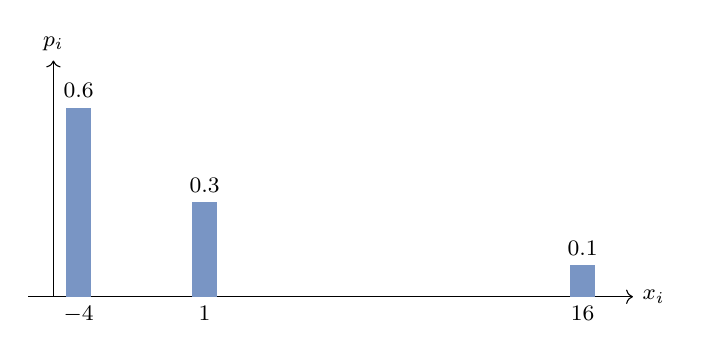
\begin{tikzpicture}[x=0.32cm,y=4cm,font=\footnotesize]
\draw[->] (-6,0)--(18,0) node[right]{$x_i$}; \draw[->] (-5,0)--(-5,0.75) node[above]{$p_i$};
\foreach \x/\p in {-4/0.6,1/0.3,16/0.1}{\fill[cDef!60] (\x-0.5,0) rectangle (\x+0.5,\p); \node[below] at (\x,0){$\x$}; \node[above] at (\x,\p){$\p$};}
\end{tikzpicture}\end{LTR}\end{center}
\end{molahada}

%================================================================
\section{الاحتمال الشرطي}
\begin{tarif}
$A$ و $B$ حادثتان مع $P(A)\neq0$. \textbf{احتمال $B$ علمًا أن $A$ محققة} هو العدد:
\[\bx{P_A(B)=\frac{P(A\cap B)}{P(A)}}\]
\end{tarif}
\begin{khassia}[دستور الاحتمالات المركبة]
\[\bx{P(A\cap B)=P(A)\times P_A(B)=P(B)\times P_B(A)}\qquad\qquad\LW{P_A\big(\overline B\big)=1-P_A(B)}\]
\end{khassia}
\begin{molahada}[التفسير]
علمًا أن $A$ محققة ، تصبح $A$ هي «مجموعة الإمكانيات الجديدة» ، ونبحث عن الجزء من $A$ الذي يحقق $B$ (أي $A\cap B$).
\begin{center}\begin{LTR}\Venn{\fill[cDef!12] (-0.55,0) circle (1); \clip (0.55,0) circle (1); \fill[cEx!45] (-0.55,0) circle (1);}{$P_A(B)$: \ar{نسبة} $A\cap B$ \ar{من} $A$}\end{LTR}\end{center}
\end{molahada}
\begin{mithal}[جدول ذو مدخلين]
مؤسسة بها $200$ عامل موزعون كما يلي ، ونختار عاملًا عشوائيًا ($H$: رجل ، $F$: امرأة ، $A$: إداري):
\begin{center}\begin{LTR}\renewcommand{\arraystretch}{1.4}
\begin{tabular}{|C|c|c|c|}\hline
\rowcolor{cSec!12} & $H$ & $F$ & \ar{المجموع}\\\hline
إداريون $A$ & $30$ & $40$ & $70$\\\hline
غير إداريين $\overline A$ & $90$ & $40$ & $130$\\\hline
المجموع & $120$ & $80$ & $200$\\\hline
\end{tabular}\end{LTR}\end{center}
\[P_F(A)=\frac{P(F\cap A)}{P(F)}=\frac{\frac{40}{200}}{\frac{80}{200}}=\frac{40}{80}=\bx{\frac12}\qquad;\qquad P_A(F)=\frac{40}{70}=\bx{\frac47}\]
\textbf{انتبه:} $P_F(A)\neq P_A(F)$.
\end{mithal}

%================================================================
\section{الشجرة المتوازنة (شجرة الاحتمالات)}
\begin{tariqa}[بناء الشجرة المتوازنة واستعمالها]
\begin{enumerate}
\item نكتب في المرحلة الأولى الحوادث $A$ و $\overline A$ (أو $A_1$ ، $A_2$ ، $\ldots$) وعلى كل فرع احتمالها.
\item نكتب في المرحلة الثانية الحوادث $B$ و $\overline B$ وعلى كل فرع \textbf{احتمالًا شرطيًا}: $P_A(B)$ ، $P_A\big(\overline B\big)$ ، $\ldots$
\item \textbf{مجموع الاحتمالات على الفروع الخارجة من نفس العقدة يساوي $1$}.
\item احتمال مسار (تقاطع) = \textbf{جداء} الاحتمالات على فروعه: $P(A\cap B)=P(A)\times P_A(B)$.
\item احتمال حادثة = \textbf{مجموع} احتمالات المسارات التي تحققها.
\end{enumerate}
\end{tariqa}
\begin{mithal}[آلتان في مصنع]
مصنع ينتج قطعًا بآلتين: الآلة $M_1$ تنتج $60\%$ من القطع و $3\%$ منها معيبة ، والآلة $M_2$ تنتج الباقي و $5\%$ منها معيبة. نختار قطعة عشوائيًا ، و $D$: «القطعة معيبة».
\par\begin{center}\begin{LTR}\begin{tikzpicture}[ev/.style={rounded rectangle,fill=cDef!12,draw=cDef,inner sep=2pt,minimum height=6mm,minimum width=7mm,font=\small},pb/.style={midway,above,sloped,font=\footnotesize,inner sep=1.5pt}]
\node[circle,fill=cDef,inner sep=1.6pt] (r) at (0,-2.10){};
\node[font=\small\bfseries,text=cSec] at (8.70,0.90){\ar{الاحتمال}};
\node[ev] (a0) at (3.20,-0.70){$M_1$};
\draw[cDef,thick] (r)--(a0) node[pb]{$0,6$};
\node[ev] (b00) at (6.40,-0.00){$D$};
\draw[cDef,thick] (a0)--(b00) node[pb]{$0,03$};
\node[font=\small] at (8.70,-0.00){$0,018$};
\node[ev] (b01) at (6.40,-1.40){$\overline D$};
\draw[cDef,thick] (a0)--(b01) node[pb]{$0,97$};
\node[font=\small] at (8.70,-1.40){$0,582$};
\node[ev] (a1) at (3.20,-3.50){$M_2$};
\draw[cDef,thick] (r)--(a1) node[pb]{$0,4$};
\node[ev] (b10) at (6.40,-2.80){$D$};
\draw[cDef,thick] (a1)--(b10) node[pb]{$0,05$};
\node[font=\small] at (8.70,-2.80){$0,02$};
\node[ev] (b11) at (6.40,-4.20){$\overline D$};
\draw[cDef,thick] (a1)--(b11) node[pb]{$0,95$};
\node[font=\small] at (8.70,-4.20){$0,38$};
\end{tikzpicture}\end{LTR}\end{center}
\[P(D)=0{,}018+0{,}02=\bx{0{,}038}\qquad;\qquad P_D(M_1)=\frac{P(M_1\cap D)}{P(D)}=\frac{0{,}018}{0{,}038}=\bx{\frac9{19}}\]
\end{mithal}

%================================================================
\section{دستور الاحتمالات الكلية}
\begin{khassia}
إذا كانت الحوادث $A_1$ ، $A_2$ ، $\ldots$ ، $A_n$ تشكل \textbf{تجزئة} لـ $\Omega$ (غير متلائمة مثنى مثنى واتحادها $\Omega$) ، فإنه من أجل كل حادثة $B$:
\[\bx{P(B)=P(A_1\cap B)+P(A_2\cap B)+\cdots+P(A_n\cap B)}\]
\[\bx{P(B)=P(A_1)\,P_{A_1}(B)+P(A_2)\,P_{A_2}(B)+\cdots+P(A_n)\,P_{A_n}(B)}\]
حالة خاصة: $\LW{P(B)=P(A)\,P_A(B)+P\big(\overline A\big)\,P_{\overline A}(B)}$.
\end{khassia}
\begin{molahada}[التفسير]
الحوادث $A_1$ ، $A_2$ ، $A_3$ تقسّم $\Omega$ ، و $B$ مقسمة إلى أجزاء $A_i\cap B$ نجمع احتمالاتها:
\begin{center}\begin{LTR}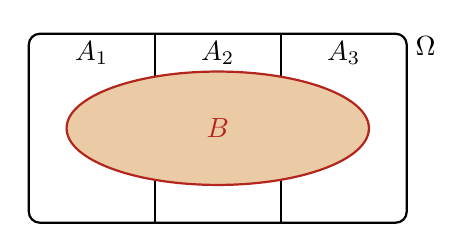
\begin{tikzpicture}[scale=0.8]
\draw[thick,rounded corners] (0,0) rectangle (6,3); \draw[thick] (2,0)--(2,3) (4,0)--(4,3);
\fill[cEx!35] (3,1.5) ellipse (2.4 and 0.9); \draw[thick,cThm] (3,1.5) ellipse (2.4 and 0.9);
\node at (1,2.7){$A_1$}; \node at (3,2.7){$A_2$}; \node at (5,2.7){$A_3$}; \node[cThm] at (3,1.5){$B$}; \node at (6.3,2.8){$\Omega$};
\end{tikzpicture}\end{LTR}\end{center}
\end{molahada}
\begin{mithal}[سحب من وعاءين]
الكيس $U_1$ يحوي $3$ كريات بيضاء و $2$ حمراوين ، والكيس $U_2$ يحوي كرية بيضاء و $4$ حمراء. نرمي قطعة نقدية متوازنة: إذا ظهر الوجه نسحب من $U_1$ ، وإلا نسحب من $U_2$. $W$: «الكرية بيضاء».
\par\begin{center}\begin{LTR}\begin{tikzpicture}[ev/.style={rounded rectangle,fill=cDef!12,draw=cDef,inner sep=2pt,minimum height=6mm,minimum width=7mm,font=\small},pb/.style={midway,above,sloped,font=\footnotesize,inner sep=1.5pt}]
\node[circle,fill=cDef,inner sep=1.6pt] (r) at (0,-2.10){};
\node[font=\small\bfseries,text=cSec] at (8.70,0.90){\ar{الاحتمال}};
\node[ev] (a0) at (3.20,-0.70){$U_1$};
\draw[cDef,thick] (r)--(a0) node[pb]{$\frac12$};
\node[ev] (b00) at (6.40,-0.00){$W$};
\draw[cDef,thick] (a0)--(b00) node[pb]{$\frac35$};
\node[font=\small] at (8.70,-0.00){$\frac3{10}$};
\node[ev] (b01) at (6.40,-1.40){$R$};
\draw[cDef,thick] (a0)--(b01) node[pb]{$\frac25$};
\node[font=\small] at (8.70,-1.40){$\frac15$};
\node[ev] (a1) at (3.20,-3.50){$U_2$};
\draw[cDef,thick] (r)--(a1) node[pb]{$\frac12$};
\node[ev] (b10) at (6.40,-2.80){$W$};
\draw[cDef,thick] (a1)--(b10) node[pb]{$\frac15$};
\node[font=\small] at (8.70,-2.80){$\frac1{10}$};
\node[ev] (b11) at (6.40,-4.20){$R$};
\draw[cDef,thick] (a1)--(b11) node[pb]{$\frac45$};
\node[font=\small] at (8.70,-4.20){$\frac25$};
\end{tikzpicture}\end{LTR}\end{center}
\[P(W)=\frac12\times\frac35+\frac12\times\frac15=\frac3{10}+\frac1{10}=\bx{\frac25}\qquad;\qquad P_W(U_1)=\frac{\frac3{10}}{\frac25}=\bx{\frac34}\]
\end{mithal}

%================================================================
\section{استقلال حادثتين}
\begin{tarif}
نقول إن الحادثتين $A$ و $B$ \textbf{مستقلتان} إذا كان: \quad $\bx{P(A\cap B)=P(A)\times P(B)}$
\par وإذا كان $P(A)\neq0$: $A$ و $B$ مستقلتان $\iff$ $\LW{P_A(B)=P(B)}$ (تحقق $A$ لا يؤثر في احتمال $B$).
\end{tarif}
\begin{khassia}
إذا كانت $A$ و $B$ مستقلتين فإن: $A$ و $\overline B$ ، و $\overline A$ و $B$ ، و $\overline A$ و $\overline B$ مستقلة أيضًا.
\end{khassia}
\begin{molahada}[انتبه]
لا نخلط بين \textbf{مستقلتين} و \textbf{غير متلائمتين}: إذا كانت $A\cap B=\varnothing$ مع $P(A)\neq0$ و $P(B)\neq0$ فإن $P(A\cap B)=0\neq P(A)P(B)$ ، أي أن الحادثتين غير المتلائمتين \textbf{غير مستقلتين}.
\par في التجارب المتتابعة مع الإرجاع (أو المستقلة) تكون نتائج المراحل مستقلة: احتمالات المرحلة الثانية لا تتغير.
\end{molahada}
\begin{mithal}
نرمي زهرة نرد غير مزيفة. $A=\{2;4;6\}$ ، $B=\{1;2\}$ ، $C=\{2;4\}$.
\par $P(A\cap B)=P(\{2\})=\dfrac16$ و $P(A)\times P(B)=\dfrac12\times\dfrac13=\dfrac16$: \bxt{$A$ و $B$ مستقلتان}.
\par $P(A\cap C)=P(\{2;4\})=\dfrac13$ و $P(A)\times P(C)=\dfrac12\times\dfrac13=\dfrac16\neq\dfrac13$: \bxt{$A$ و $C$ غير مستقلتين}.
\end{mithal}

%================================================================
\section{تمارين محلولة}
\begin{tmr}
أجرى بنك دراسة على زبائنه: $60\%$ منهم يملكون دفتر ادخار $(E)$ ، و $30\%$ من هؤلاء استفادوا من قرض $(C)$ ، بينما $50\%$ من الذين لا يملكون دفتر ادخار استفادوا من قرض. نختار زبونًا عشوائيًا.
\QQ{1} أنجز شجرة الاحتمالات المتوازنة التي تنمذج هذه الوضعية.
\QQ{2} احسب $P(E\cap C)$ ، ثم بيّن أن $P(C)=0{,}38$.
\QQ{3} علمًا أن الزبون استفاد من قرض ، ما احتمال أن يملك دفتر ادخار؟
\QQ{4} هل الحادثتان $E$ و $C$ مستقلتان؟
\QQ{5} يحقق البنك ربحًا $X$ (بآلاف الدنانير) من كل زبون: $300$ إذا كان له دفتر وقرض ، $100$ إذا كان له دفتر فقط ، $200$ إذا كان له قرض فقط ، و $0$ في الحالة الأخرى. عيّن قانون احتمال $X$ ، ثم احسب $E(X)$ و $\sigma(X)$.
\end{tmr}
\begin{hal}
\QQ{1} $P\big(\overline E\big)=0{,}4$ ، $P_E\big(\overline C\big)=0{,}7$ ، $P_{\overline E}\big(\overline C\big)=0{,}5$:
\par\begin{center}\begin{LTR}\begin{tikzpicture}[ev/.style={rounded rectangle,fill=cDef!12,draw=cDef,inner sep=2pt,minimum height=6mm,minimum width=7mm,font=\small},pb/.style={midway,above,sloped,font=\footnotesize,inner sep=1.5pt}]
\node[circle,fill=cDef,inner sep=1.6pt] (r) at (0,-2.10){};
\node[font=\small\bfseries,text=cSec] at (8.70,0.90){\ar{الاحتمال}};
\node[ev] (a0) at (3.20,-0.70){$E$};
\draw[cDef,thick] (r)--(a0) node[pb]{$0,6$};
\node[ev] (b00) at (6.40,-0.00){$C$};
\draw[cDef,thick] (a0)--(b00) node[pb]{$0,3$};
\node[font=\small] at (8.70,-0.00){$0,18$};
\node[ev] (b01) at (6.40,-1.40){$\overline C$};
\draw[cDef,thick] (a0)--(b01) node[pb]{$0,7$};
\node[font=\small] at (8.70,-1.40){$0,42$};
\node[ev] (a1) at (3.20,-3.50){$\overline E$};
\draw[cDef,thick] (r)--(a1) node[pb]{$0,4$};
\node[ev] (b10) at (6.40,-2.80){$C$};
\draw[cDef,thick] (a1)--(b10) node[pb]{$0,5$};
\node[font=\small] at (8.70,-2.80){$0,2$};
\node[ev] (b11) at (6.40,-4.20){$\overline C$};
\draw[cDef,thick] (a1)--(b11) node[pb]{$0,5$};
\node[font=\small] at (8.70,-4.20){$0,2$};
\end{tikzpicture}\end{LTR}\end{center}
\QQ{2} $P(E\cap C)=0{,}6\times0{,}3=\bx{0{,}18}$ \ ، \ $P(C)=0{,}18+0{,}4\times0{,}5=0{,}18+0{,}2=\bx{0{,}38}$ (دستور الاحتمالات الكلية).
\QQ{3} $P_C(E)=\dfrac{0{,}18}{0{,}38}=\bx{\frac9{19}}$
\QQ{4} $P(E)\times P(C)=0{,}6\times0{,}38=0{,}228\neq0{,}18$: \bxt{$E$ و $C$ غير مستقلتين}.
\QQ{5}
\begin{center}\begin{LTR}\renewcommand{\arraystretch}{1.5}
\begin{tabular}{|c|c|c|c|c|C|}\hline
\rowcolor{cSec!12}$x_i$ & $0$ & $100$ & $200$ & $300$ & المجموع\\\hline
$P(X=x_i)$ & $0{,}2$ & $0{,}42$ & $0{,}2$ & $0{,}18$ & $1$\\\hline
\end{tabular}\end{LTR}\end{center}
\[E(X)=0+42+40+54=\bx{136}\]
\[V(X)=4200+8000+16200-136^2=28400-18496=9904\]
\[\sigma(X)=\sqrt{9904}\approx\bx{99{,}52}\]
\end{hal}
\begin{tmr}
كيس يحوي $3$ كريات حمراء و $2$ خضراوين. نسحب كريتين على التوالي.
\QQ{1} \textbf{مع الإرجاع:} $X$ عدد الكريات الحمراء المسحوبة. أنجز الشجرة ، ثم عيّن قانون احتمال $X$ واحسب $E(X)$ و $V(X)$.
\QQ{2} \textbf{دون إرجاع:} احسب احتمال سحب كريتين من نفس اللون ، واحتمال أن تكون الكرية الثانية حمراء ، ثم احتمال أن تكون الأولى حمراء علمًا أن الثانية حمراء.
\end{tmr}
\begin{hal}
\QQ{1} مع الإرجاع ، السحبان مستقلان والاحتمالات لا تتغير:
\par\begin{center}\begin{LTR}\begin{tikzpicture}[ev/.style={rounded rectangle,fill=cDef!12,draw=cDef,inner sep=2pt,minimum height=6mm,minimum width=7mm,font=\small},pb/.style={midway,above,sloped,font=\footnotesize,inner sep=1.5pt}]
\node[circle,fill=cDef,inner sep=1.6pt] (r) at (0,-2.10){};
\node[font=\small\bfseries,text=cSec] at (8.70,0.90){\ar{الاحتمال}};
\node[ev] (a0) at (3.20,-0.70){$R$};
\draw[cDef,thick] (r)--(a0) node[pb]{$\frac35$};
\node[ev] (b00) at (6.40,-0.00){$R$};
\draw[cDef,thick] (a0)--(b00) node[pb]{$\frac35$};
\node[font=\small] at (8.70,-0.00){$\frac9{25}$};
\node[ev] (b01) at (6.40,-1.40){$G$};
\draw[cDef,thick] (a0)--(b01) node[pb]{$\frac25$};
\node[font=\small] at (8.70,-1.40){$\frac6{25}$};
\node[ev] (a1) at (3.20,-3.50){$G$};
\draw[cDef,thick] (r)--(a1) node[pb]{$\frac25$};
\node[ev] (b10) at (6.40,-2.80){$R$};
\draw[cDef,thick] (a1)--(b10) node[pb]{$\frac35$};
\node[font=\small] at (8.70,-2.80){$\frac6{25}$};
\node[ev] (b11) at (6.40,-4.20){$G$};
\draw[cDef,thick] (a1)--(b11) node[pb]{$\frac25$};
\node[font=\small] at (8.70,-4.20){$\frac4{25}$};
\end{tikzpicture}\end{LTR}\end{center}
\begin{center}\begin{LTR}\renewcommand{\arraystretch}{1.6}
\begin{tabular}{|c|c|c|c|C|}\hline
\rowcolor{cSec!12}$x_i$ & $0$ & $1$ & $2$ & المجموع\\\hline
$P(X=x_i)$ & $\frac4{25}$ & $\frac{12}{25}$ & $\frac9{25}$ & $1$\\\hline
\end{tabular}\end{LTR}\end{center}
\[E(X)=0+\frac{12}{25}+\frac{18}{25}=\bx{\frac65}\qquad;\qquad V(X)=\frac{12}{25}+\frac{36}{25}-\frac{36}{25}=\bx{\frac{12}{25}}\]
\QQ{2} دون إرجاع ، تتغير الاحتمالات في المرحلة الثانية:
\par\begin{center}\begin{LTR}\begin{tikzpicture}[ev/.style={rounded rectangle,fill=cDef!12,draw=cDef,inner sep=2pt,minimum height=6mm,minimum width=7mm,font=\small},pb/.style={midway,above,sloped,font=\footnotesize,inner sep=1.5pt}]
\node[circle,fill=cDef,inner sep=1.6pt] (r) at (0,-2.10){};
\node[font=\small\bfseries,text=cSec] at (8.70,0.90){\ar{الاحتمال}};
\node[ev] (a0) at (3.20,-0.70){$R$};
\draw[cDef,thick] (r)--(a0) node[pb]{$\frac35$};
\node[ev] (b00) at (6.40,-0.00){$R$};
\draw[cDef,thick] (a0)--(b00) node[pb]{$\frac24$};
\node[font=\small] at (8.70,-0.00){$\frac3{10}$};
\node[ev] (b01) at (6.40,-1.40){$G$};
\draw[cDef,thick] (a0)--(b01) node[pb]{$\frac24$};
\node[font=\small] at (8.70,-1.40){$\frac3{10}$};
\node[ev] (a1) at (3.20,-3.50){$G$};
\draw[cDef,thick] (r)--(a1) node[pb]{$\frac25$};
\node[ev] (b10) at (6.40,-2.80){$R$};
\draw[cDef,thick] (a1)--(b10) node[pb]{$\frac34$};
\node[font=\small] at (8.70,-2.80){$\frac3{10}$};
\node[ev] (b11) at (6.40,-4.20){$G$};
\draw[cDef,thick] (a1)--(b11) node[pb]{$\frac14$};
\node[font=\small] at (8.70,-4.20){$\frac1{10}$};
\end{tikzpicture}\end{LTR}\end{center}
\[P(RR)+P(GG)=\frac3{10}+\frac1{10}=\bx{\frac25}\]
\[P(R_2)=\frac3{10}+\frac3{10}=\bx{\frac35}\qquad;\qquad P_{R_2}(R_1)=\frac{\frac3{10}}{\frac35}=\bx{\frac12}\]
\end{hal}

%================================================================
\clearpage
\section{خلاصة الطرائق}
\begin{BOX}{cMeth}{الطريقة حسب المطلوب}
\begin{center}
\renewcommand{\arraystretch}{1.5}
\begin{tabular}{|p{0.62\textwidth}|p{0.3\textwidth}|}\hline
\rowcolor{cSec!12} \textbf{الطريقة} & \textbf{المطلوب}\\\hline
$P(A)=\dfrac{\text{card}\,A}{\text{card}\,\Omega}$ (نعدّ الحالات بقائمة أو بجدول ذي مدخلين). & احتمال في حالة تساوي الاحتمال\\\hline
$P\big(\overline A\big)=1-P(A)$ ، خاصة لـ «على الأقل». & احتمال الحادثة العكسية\\\hline
نعيّن القيم $x_i$ ثم $p_i$ في جدول ، ونتحقق أن $\sum p_i=1$. & قانون احتمال متغير عشوائي\\\hline
$E(X)=\sum x_ip_i$ ، $V(X)=\sum x_i^2p_i-E(X)^2$ ، $\sigma=\sqrt V$. & الأمل والتباين والانحراف المعياري\\\hline
$E(X)>0$: في صالح اللاعب ؛ $E(X)=0$: لعبة عادلة. & تفسير الأمل الرياضياتي\\\hline
مرحلة أولى: $P(A)$ ؛ مرحلة ثانية: احتمالات شرطية ؛ مجموع الفروع من نفس العقدة $=1$. & بناء الشجرة المتوازنة\\\hline
جداء الاحتمالات على المسار: $P(A\cap B)=P(A)\times P_A(B)$. & احتمال تقاطع\\\hline
مجموع احتمالات المسارات: $P(B)=P(A)P_A(B)+P\big(\overline A\big)P_{\overline A}(B)$. & احتمال حادثة في المرحلة الثانية (الاحتمالات الكلية)\\\hline
$P_B(A)=\dfrac{P(A\cap B)}{P(B)}$. & احتمال «علمًا أن»\\\hline
نقارن $P(A\cap B)$ و $P(A)\times P(B)$. & استقلال حادثتين\\\hline
\end{tabular}
\end{center}
\end{BOX}
\end{document}
